% Created by tikzDevice version 0.12.6 on 2024-03-27 07:53:43
% !TEX encoding = UTF-8 Unicode
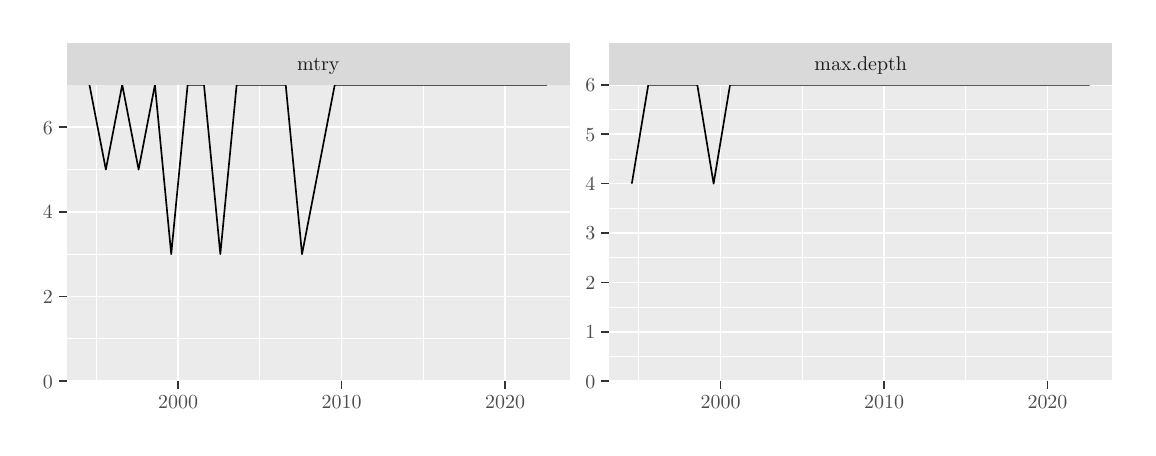
\begin{tikzpicture}[x=1pt,y=1pt]
\definecolor{fillColor}{RGB}{255,255,255}
\path[use as bounding box,fill=fillColor,fill opacity=0.00] (0,0) rectangle (397.48,144.54);
\begin{scope}
\path[clip] (  0.00,  0.00) rectangle (397.48,144.54);
\definecolor{drawColor}{RGB}{255,255,255}
\definecolor{fillColor}{RGB}{255,255,255}

\path[draw=drawColor,line width= 0.6pt,line join=round,line cap=round,fill=fillColor] (  0.00,  0.00) rectangle (397.48,144.54);
\end{scope}
\begin{scope}
\path[clip] ( 14.05, 16.81) rectangle (195.99,123.88);
\definecolor{fillColor}{gray}{0.92}

\path[fill=fillColor] ( 14.05, 16.81) rectangle (195.99,123.88);
\definecolor{drawColor}{RGB}{255,255,255}

\path[draw=drawColor,line width= 0.3pt,line join=round] ( 14.05, 32.10) --
	(195.99, 32.10);

\path[draw=drawColor,line width= 0.3pt,line join=round] ( 14.05, 62.70) --
	(195.99, 62.70);

\path[draw=drawColor,line width= 0.3pt,line join=round] ( 14.05, 93.29) --
	(195.99, 93.29);

\path[draw=drawColor,line width= 0.3pt,line join=round] ( 14.05,123.88) --
	(195.99,123.88);

\path[draw=drawColor,line width= 0.3pt,line join=round] ( 24.83, 16.81) --
	( 24.83,123.88);

\path[draw=drawColor,line width= 0.3pt,line join=round] ( 83.91, 16.81) --
	( 83.91,123.88);

\path[draw=drawColor,line width= 0.3pt,line join=round] (142.99, 16.81) --
	(142.99,123.88);

\path[draw=drawColor,line width= 0.6pt,line join=round] ( 14.05, 16.81) --
	(195.99, 16.81);

\path[draw=drawColor,line width= 0.6pt,line join=round] ( 14.05, 47.40) --
	(195.99, 47.40);

\path[draw=drawColor,line width= 0.6pt,line join=round] ( 14.05, 77.99) --
	(195.99, 77.99);

\path[draw=drawColor,line width= 0.6pt,line join=round] ( 14.05,108.59) --
	(195.99,108.59);

\path[draw=drawColor,line width= 0.6pt,line join=round] ( 54.37, 16.81) --
	( 54.37,123.88);

\path[draw=drawColor,line width= 0.6pt,line join=round] (113.46, 16.81) --
	(113.46,123.88);

\path[draw=drawColor,line width= 0.6pt,line join=round] (172.52, 16.81) --
	(172.52,123.88);
\definecolor{drawColor}{RGB}{0,0,0}

\path[draw=drawColor,line width= 0.6pt,line join=round] ( 22.32,123.88) --
	( 28.25, 93.29) --
	( 34.17,123.88) --
	( 40.08, 93.29) --
	( 45.98,123.88) --
	( 51.87, 62.70) --
	( 57.80,123.88) --
	( 63.71,123.88) --
	( 69.61, 62.70) --
	( 75.51,123.88) --
	( 81.42,123.88) --
	( 87.30,123.88) --
	( 93.24,123.88) --
	( 99.14, 62.70) --
	(105.06, 93.29) --
	(110.96,123.88) --
	(116.85,123.88) --
	(122.74,123.88) --
	(128.69,123.88) --
	(134.59,123.88) --
	(140.50,123.88) --
	(146.40,123.88) --
	(152.29,123.88) --
	(158.22,123.88) --
	(164.13,123.88) --
	(170.03,123.88) --
	(175.95,123.88) --
	(181.84,123.88) --
	(187.72,123.88);
\end{scope}
\begin{scope}
\path[clip] (210.04, 16.81) rectangle (391.98,123.88);
\definecolor{fillColor}{gray}{0.92}

\path[fill=fillColor] (210.04, 16.81) rectangle (391.98,123.88);
\definecolor{drawColor}{RGB}{255,255,255}

\path[draw=drawColor,line width= 0.3pt,line join=round] (210.04, 25.73) --
	(391.98, 25.73);

\path[draw=drawColor,line width= 0.3pt,line join=round] (210.04, 43.58) --
	(391.98, 43.58);

\path[draw=drawColor,line width= 0.3pt,line join=round] (210.04, 61.42) --
	(391.98, 61.42);

\path[draw=drawColor,line width= 0.3pt,line join=round] (210.04, 79.27) --
	(391.98, 79.27);

\path[draw=drawColor,line width= 0.3pt,line join=round] (210.04, 97.11) --
	(391.98, 97.11);

\path[draw=drawColor,line width= 0.3pt,line join=round] (210.04,114.96) --
	(391.98,114.96);

\path[draw=drawColor,line width= 0.3pt,line join=round] (220.83, 16.81) --
	(220.83,123.88);

\path[draw=drawColor,line width= 0.3pt,line join=round] (279.91, 16.81) --
	(279.91,123.88);

\path[draw=drawColor,line width= 0.3pt,line join=round] (338.98, 16.81) --
	(338.98,123.88);

\path[draw=drawColor,line width= 0.6pt,line join=round] (210.04, 16.81) --
	(391.98, 16.81);

\path[draw=drawColor,line width= 0.6pt,line join=round] (210.04, 34.65) --
	(391.98, 34.65);

\path[draw=drawColor,line width= 0.6pt,line join=round] (210.04, 52.50) --
	(391.98, 52.50);

\path[draw=drawColor,line width= 0.6pt,line join=round] (210.04, 70.34) --
	(391.98, 70.34);

\path[draw=drawColor,line width= 0.6pt,line join=round] (210.04, 88.19) --
	(391.98, 88.19);

\path[draw=drawColor,line width= 0.6pt,line join=round] (210.04,106.04) --
	(391.98,106.04);

\path[draw=drawColor,line width= 0.6pt,line join=round] (210.04,123.88) --
	(391.98,123.88);

\path[draw=drawColor,line width= 0.6pt,line join=round] (250.37, 16.81) --
	(250.37,123.88);

\path[draw=drawColor,line width= 0.6pt,line join=round] (309.45, 16.81) --
	(309.45,123.88);

\path[draw=drawColor,line width= 0.6pt,line join=round] (368.51, 16.81) --
	(368.51,123.88);
\definecolor{drawColor}{RGB}{0,0,0}

\path[draw=drawColor,line width= 0.6pt,line join=round] (218.31, 88.19) --
	(224.25,123.88) --
	(230.17,123.88) --
	(236.07,123.88) --
	(241.97,123.88) --
	(247.86, 88.19) --
	(253.80,123.88) --
	(259.70,123.88) --
	(265.60,123.88) --
	(271.51,123.88) --
	(277.41,123.88) --
	(283.30,123.88) --
	(289.23,123.88) --
	(295.13,123.88) --
	(301.05,123.88) --
	(306.96,123.88) --
	(312.84,123.88) --
	(318.73,123.88) --
	(324.68,123.88) --
	(330.59,123.88) --
	(336.49,123.88) --
	(342.39,123.88) --
	(348.28,123.88) --
	(354.21,123.88) --
	(360.12,123.88) --
	(366.02,123.88) --
	(371.94,123.88) --
	(377.83,123.88) --
	(383.71,123.88);
\end{scope}
\begin{scope}
\path[clip] ( 14.05,123.88) rectangle (195.99,139.04);
\definecolor{fillColor}{gray}{0.85}

\path[fill=fillColor] ( 14.05,123.88) rectangle (195.99,139.04);
\definecolor{drawColor}{gray}{0.10}

\node[text=drawColor,anchor=base,inner sep=0pt, outer sep=0pt, scale=  0.72] at (105.02,128.98) {mtry};
\end{scope}
\begin{scope}
\path[clip] (210.04,123.88) rectangle (391.98,139.04);
\definecolor{fillColor}{gray}{0.85}

\path[fill=fillColor] (210.04,123.88) rectangle (391.98,139.04);
\definecolor{drawColor}{gray}{0.10}

\node[text=drawColor,anchor=base,inner sep=0pt, outer sep=0pt, scale=  0.72] at (301.01,128.98) {max.depth};
\end{scope}
\begin{scope}
\path[clip] (  0.00,  0.00) rectangle (397.48,144.54);
\definecolor{drawColor}{gray}{0.20}

\path[draw=drawColor,line width= 0.6pt,line join=round] ( 54.37, 14.06) --
	( 54.37, 16.81);

\path[draw=drawColor,line width= 0.6pt,line join=round] (113.46, 14.06) --
	(113.46, 16.81);

\path[draw=drawColor,line width= 0.6pt,line join=round] (172.52, 14.06) --
	(172.52, 16.81);
\end{scope}
\begin{scope}
\path[clip] (  0.00,  0.00) rectangle (397.48,144.54);
\definecolor{drawColor}{gray}{0.30}

\node[text=drawColor,anchor=base,inner sep=0pt, outer sep=0pt, scale=  0.72] at ( 54.37,  6.90) {2000};

\node[text=drawColor,anchor=base,inner sep=0pt, outer sep=0pt, scale=  0.72] at (113.46,  6.90) {2010};

\node[text=drawColor,anchor=base,inner sep=0pt, outer sep=0pt, scale=  0.72] at (172.52,  6.90) {2020};
\end{scope}
\begin{scope}
\path[clip] (  0.00,  0.00) rectangle (397.48,144.54);
\definecolor{drawColor}{gray}{0.20}

\path[draw=drawColor,line width= 0.6pt,line join=round] (250.37, 14.06) --
	(250.37, 16.81);

\path[draw=drawColor,line width= 0.6pt,line join=round] (309.45, 14.06) --
	(309.45, 16.81);

\path[draw=drawColor,line width= 0.6pt,line join=round] (368.51, 14.06) --
	(368.51, 16.81);
\end{scope}
\begin{scope}
\path[clip] (  0.00,  0.00) rectangle (397.48,144.54);
\definecolor{drawColor}{gray}{0.30}

\node[text=drawColor,anchor=base,inner sep=0pt, outer sep=0pt, scale=  0.72] at (250.37,  6.90) {2000};

\node[text=drawColor,anchor=base,inner sep=0pt, outer sep=0pt, scale=  0.72] at (309.45,  6.90) {2010};

\node[text=drawColor,anchor=base,inner sep=0pt, outer sep=0pt, scale=  0.72] at (368.51,  6.90) {2020};
\end{scope}
\begin{scope}
\path[clip] (  0.00,  0.00) rectangle (397.48,144.54);
\definecolor{drawColor}{gray}{0.30}

\node[text=drawColor,anchor=base east,inner sep=0pt, outer sep=0pt, scale=  0.72] at (205.09, 14.33) {0};

\node[text=drawColor,anchor=base east,inner sep=0pt, outer sep=0pt, scale=  0.72] at (205.09, 32.17) {1};

\node[text=drawColor,anchor=base east,inner sep=0pt, outer sep=0pt, scale=  0.72] at (205.09, 50.02) {2};

\node[text=drawColor,anchor=base east,inner sep=0pt, outer sep=0pt, scale=  0.72] at (205.09, 67.87) {3};

\node[text=drawColor,anchor=base east,inner sep=0pt, outer sep=0pt, scale=  0.72] at (205.09, 85.71) {4};

\node[text=drawColor,anchor=base east,inner sep=0pt, outer sep=0pt, scale=  0.72] at (205.09,103.56) {5};

\node[text=drawColor,anchor=base east,inner sep=0pt, outer sep=0pt, scale=  0.72] at (205.09,121.40) {6};
\end{scope}
\begin{scope}
\path[clip] (  0.00,  0.00) rectangle (397.48,144.54);
\definecolor{drawColor}{gray}{0.20}

\path[draw=drawColor,line width= 0.6pt,line join=round] (207.29, 16.81) --
	(210.04, 16.81);

\path[draw=drawColor,line width= 0.6pt,line join=round] (207.29, 34.65) --
	(210.04, 34.65);

\path[draw=drawColor,line width= 0.6pt,line join=round] (207.29, 52.50) --
	(210.04, 52.50);

\path[draw=drawColor,line width= 0.6pt,line join=round] (207.29, 70.34) --
	(210.04, 70.34);

\path[draw=drawColor,line width= 0.6pt,line join=round] (207.29, 88.19) --
	(210.04, 88.19);

\path[draw=drawColor,line width= 0.6pt,line join=round] (207.29,106.04) --
	(210.04,106.04);

\path[draw=drawColor,line width= 0.6pt,line join=round] (207.29,123.88) --
	(210.04,123.88);
\end{scope}
\begin{scope}
\path[clip] (  0.00,  0.00) rectangle (397.48,144.54);
\definecolor{drawColor}{gray}{0.30}

\node[text=drawColor,anchor=base east,inner sep=0pt, outer sep=0pt, scale=  0.72] at (  9.10, 14.33) {0};

\node[text=drawColor,anchor=base east,inner sep=0pt, outer sep=0pt, scale=  0.72] at (  9.10, 44.92) {2};

\node[text=drawColor,anchor=base east,inner sep=0pt, outer sep=0pt, scale=  0.72] at (  9.10, 75.51) {4};

\node[text=drawColor,anchor=base east,inner sep=0pt, outer sep=0pt, scale=  0.72] at (  9.10,106.11) {6};
\end{scope}
\begin{scope}
\path[clip] (  0.00,  0.00) rectangle (397.48,144.54);
\definecolor{drawColor}{gray}{0.20}

\path[draw=drawColor,line width= 0.6pt,line join=round] ( 11.30, 16.81) --
	( 14.05, 16.81);

\path[draw=drawColor,line width= 0.6pt,line join=round] ( 11.30, 47.40) --
	( 14.05, 47.40);

\path[draw=drawColor,line width= 0.6pt,line join=round] ( 11.30, 77.99) --
	( 14.05, 77.99);

\path[draw=drawColor,line width= 0.6pt,line join=round] ( 11.30,108.59) --
	( 14.05,108.59);
\end{scope}
\end{tikzpicture}
